\section{Testy wydajnościowe}

Celem niniejszego podrozdziału jest przeprowadzenie testów wydajnościowych dla obu typów wielomianów. PolynomialMap i~PolynomialVector to bardzo podobne klasy, których struktura została jednak oparta na odmiennych podejściach. PolynomialMap opiera się na przechowywaniu wyłącznie niezerowych współczynników wielomianu. Z kolei PolynomialVector jako kontenera danych używa wektora, co wymusza przechowywanie wszystkich współczynników, także zerowych.

Zestaw przeprowadzonych testów dobrałem tak, by pozwoliły one na zbadanie zupełnie różnych przypadków. Teoretycznie bowiem obiekty typu PolynomialMap powinny być dużo wydajniejsze dla wielomianów rzadkich. Z drugiej strony, w~przypadku wielomianów gęstych różnica pomiędzy obiema klasami powinna być zdecydowanie mniejsza. Wydaje się, że w~takiej sytuacji niewielką przewagę powinna mieć klasa wielomianu oparta o~użycie tablicy. W~tym miejscu warto przypomnieć, że wielomiany nazywami gęstymi, jeżeli większość współczynników jest niezerowa, zaś wielomiany, których większość współczynników stanowią zera to wielomiany rzadkie.

Zapoznajmy się więc z~poniższymi testami, by zweryfikowac przedstawioną wyżej tezę.

\subsection{Testowanie wielomianów gęstych}

\subsubsection{Wielomiany stopnia parzystego}

Pierwszym przypadkiem testowym będzie sprawdzenie czasów znajdowania pierwiastków dla takich wielomianów, których wszystkie współczynniki są równe $1$. Testowane wielomiany można przedstawić wzorem:
\begin{equation*}
W(x) = x^k + x^{k-1} + x^{k-2} + ... + x^2 + x + 1\text{, gdzie } k \text{ jest stopniem wielomianu } W \text {.}
\end{equation*}


W przypadku, gdy stopień wielomianu jest liczbą parzystą, a~jego wszystkie współczynniki są równe $1$, wielomian nie posiada pierwiastków rzeczywistych. Sprawdźmy ile czasu zajmie każdej ze struktur stwierdzenie braku pierwiastków rzeczywistych dla wielomianów powyższej postaci.

\begin{table}[H]
	\begin{tabular}{ |p{4cm}|p{2.75cm}|p{2.75cm}|p{3.5cm}|} 
		\hline
		Testowany wielomian & Czas dla PolynomialMap [s] & Czas dla PolynomialVector [s] & Współczynnik czasów \\
		\hline
		$W(x) = x^{10} + x^9 + ... + x + 1$ & 0.077 & 0.079 & 1.026 \\
		$W(x) = x^{20} + x^{19} + ... + x + 1$ & 0.29 & 0.291 & 1.003 \\
		$W(x) = x^{40} + x^{39} + ... + x + 1$ & 1.176 & 1.174 & 0.998 \\
		$W(x) = x^{80} + x^{79} + ... + x + 1$ & 5.046 & 5.048 & 1 \\
		$W(x) = x^{160} + x^{159} + ... + x + 1$  & 22.879 & 23.047 & 1.007 \\
		$W(x) = x^{320} + x^{319} + ... + x + 1$  & 114.311 & 114.382 & 1.001 \\
		\hline
	\end{tabular}
	\caption{Porównanie czasów znajdowania pierwiastków dla gęstych wielomianów parzystego stopnia. Źródło: opracowanie własne.}
\end{table}

W tabeli dla każdego przeprowadzonego testu została dodana wartość współczynnika czasów, zdefiniowa jako iloraz czasu działania typu PolynomialVector i~PolynomialMap. Ich wartość dla wszystkich testów jest bliska lub równa $1$. Na tej podstawie łatwo zauważyć, że czasy znajdowania pierwiastków wielomianów dla obu struktur jest praktycznie identyczny. Z tego powodu poniższy wykres pokazuje dwie praktycznie w~całości pokrywające się linie, oznaczające czas działania obu typoów wielomianów w~zależności od testowanego stopnia.

\begin{figure}[H]
	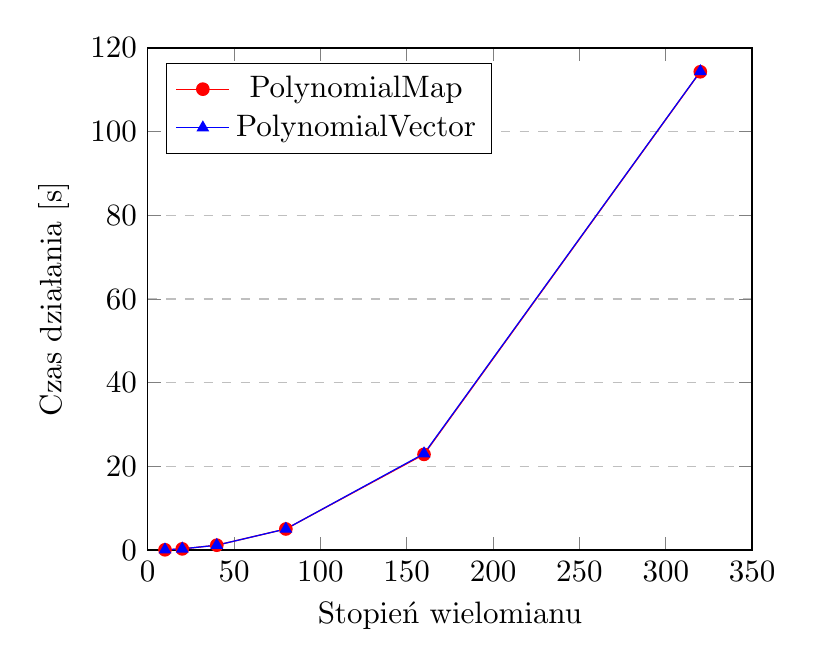
\begin{tikzpicture}[scale=1.12]
	\begin{axis}[
	xlabel={Stopień wielomianu},
	ylabel={Czas działania [s]},
	xmin=0,xmax=350,
	ymin=0,ymax=120,
	ymajorgrids=true,grid style=dashed,
	legend pos=north west
	]
	
	\addplot[color=red,mark=*]
	coordinates {
		(10, 0.077)
		(20, 0.29)
		(40, 1.176)
		(80, 5.046)
		(160, 22.879)
		(320, 114.311)
	};
	
	\addplot[color=blue,mark=triangle*]
	coordinates {
		(10, 0.079)
		(20, 0.291)
		(40, 1.174)
		(80, 5.048)
		(160, 23.047)
		(320, 114.382)	
	};
	
	\legend{PolynomialMap, PolynomialVector}
	\end{axis}
	\end{tikzpicture}
	\caption{Czasy znajdowania pierwiastków dla gęstych wielomianów parzystego stopnia. Źródło: opracowanie własne.}
\end{figure}

\subsubsection{Wielomiany stopnia nieparzystego}

To analogiczny test w~porównaniu z~poprzednim, jednak w~tym przypadku stopień wielomianu jest nieparzysty. Wpływa to na liczbę pierwiastków rzeczywistych wielomianu, zwiększając ją o~$1$. Sprawdźmy, czy wyniki będą podobne do tych uzyskanych dla wielomianów stopnia parzystego.

\begin{table}[H]
	\begin{tabular}{ |p{4cm}|p{2.75cm}|p{2.75cm}|p{3.5cm}|} 
		\hline
		Testowany wielomian & Czas dla PolynomialMap [s] & Czas dla PolynomialVector [s] & Współczynnik czasów \\
		\hline
		$W(x) = x^{11} + x^{10} + ... + x + 1$ & 3.224 & 3.269 & 1.014 \\
		$W(x) = x^{21} + x^{20} + ... + x + 1$ & 13.384 & 13.548 & 1.012 \\
		$W(x) = x^{41} + x^{40} + ... + x + 1$ & 57.336 & 57.336 & 1 \\
		$W(x) = x^{81} + x^{80} + ... + x + 1$ & 260.175 & 261.915 & 1.007 \\
		$W(x) = x^{161} + x^{160} + ... + x + 1$  & 1286.409 & 1286.261 & 1 \\
		$W(x) = x^{321} + x^{320} + ... + x + 1$  & 7190.234 & 7205.386 & 1.002 \\
		\hline
	\end{tabular}
	\caption{Porównanie czasów znajdowania pierwiastków dla gęstych wielomianów nieparzystego stopnia. Źródło: opracowanie własne.}
\end{table}

Także i~w~tym przypadku porównywane czasy działania są prawie identyczne. Ich wartości w~zależności od stopnia testowanego wielomianu zostały przedstawione na poniższym wykresie.

\begin{figure}[H]
	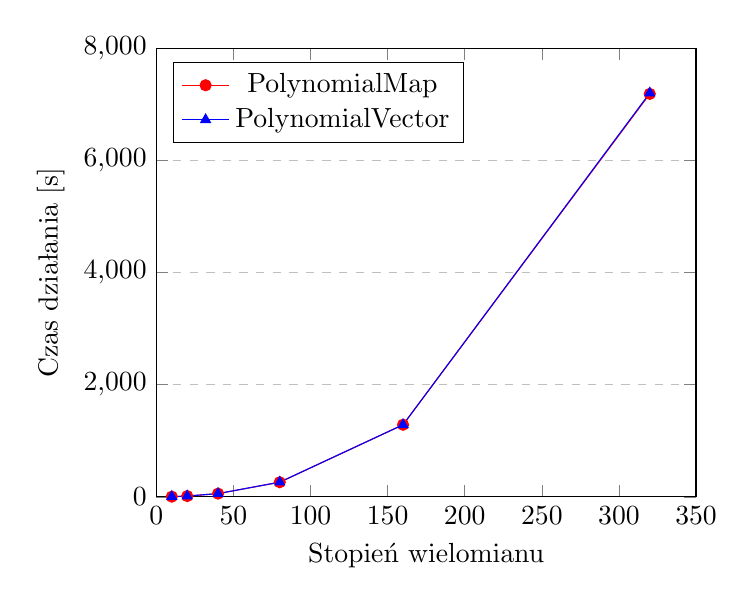
\begin{tikzpicture}[scale=1]
	\begin{axis}[
	xlabel={Stopień wielomianu},
	ylabel={Czas działania [s]},
	xmin=0,xmax=350,
	ymin=0,ymax=8000,
	ymajorgrids=true,grid style=dashed,
	legend pos=north west
	]
	
	\addplot[color=red,mark=*]
	coordinates {
		(10, 3.224)
		(20, 13.384)
		(40, 57.336)
		(80, 260.175)
		(160, 1286.409)
		(320, 7190.234)
	};
	
	\addplot[color=blue,mark=triangle*]
	coordinates {
		(10, 3.269)
		(20, 13.548)
		(40, 57.336)
		(80, 261.915)
		(160, 1286.261)
		(320, 7205.386)	
	};

	\legend{PolynomialMap, PolynomialVector}
	\end{axis}
	\end{tikzpicture}
	\caption{Czas znajdowania pierwiastków dla wielomianów zawierających kolejne pierwiastki całkowite. Źródło: opracowanie własne.}
\end{figure}

Porównując wartości uzyskane dla wielomianów stopnia parzystego i~nieparzystego uwagę zwraca fakt, że uzyskane czasy dla wielomianów stopnia nieparzystego, czyli takich posiadających przynajmniej jeden pierwiastek rzeczywistych są kilkadziesiąt razy większe niż dla wielomianów stopnia parzystego. Oznacza to, że liczba pierwiastków rzeczywistych ma ogromny wpływ na czas działania algorytmu ich znajdowania. Testy potwierdzają, że sytuacja taka jest obserwowana niezależnie od typu użytej struktury wielomianu.
